% Keep the supplied class unchanged. pdfLaTeX uses its original spot colours.
% Tectonic/XeTeX preview uses the identical declared CMYK colour because the
% template's 2006 spotcolor package only implements pdfTeX primitives.
\RequirePackage{iftex}
\ifXeTeX
  \RequirePackage[T1]{fontenc}
  \RequirePackage{color}
  \makeatletter
  \@namedef{ver@spotcolor.sty}{2026/09/16 XeTeX preview compatibility}
  \newcommand\NewSpotColorSpace[1]{}
  \newcommand\AddSpotColor[4]{}
  \newcommand\SetPageColorSpace[1]{}
  \def\color@spotcolor#1#2{\color@cmyk#1{1,0.3,0,0.2}}
  \makeatother
\fi

\documentclass[nolineno]{ieeeaccess}
\usepackage{cite}
\usepackage{amsmath,amssymb,amsfonts}
\usepackage{graphicx,booktabs,tabularx,array}
\usepackage{textcomp,xurl}
\usepackage[hidelinks]{hyperref}
\usepackage{iftex,etoolbox,needspace,placeins}
\makeatletter
\InputIfFileExists{t1pcr.fd}{}{}
\DeclareFontShape{T1}{pcr}{n}{n}{<->ssub*pcr/m/n}{}
\DeclareFontShape{T1}{formata}{m}{sl}{<->ssub*formata/m/it}{}
\makeatother
\makeatletter
% Keep the supplied photo biographies together without elastic vertical gaps.
\def\@IEEEBIOskipN{1.25\baselineskip}
\expandafter\patchcmd\csname\string\IEEEbiography\endcsname
  {\vskip \@IEEEBIOskipN plus 1fil minus 0\baselineskip}
  {\vskip \@IEEEBIOskipN}{}{}
\newcommand{\submissionfooter}{\hbox to\textwidth{\hfill\footerpagefont\thepage}}
\apptocmd{\ps@titlepage}{\let\@oddfoot\submissionfooter\let\@evenfoot\submissionfooter}{}{}
\apptocmd{\ps@headings}{\let\@oddfoot\submissionfooter\let\@evenfoot\submissionfooter}{}{}
\patchcmd{\@maketitle}{Digital Object Identifier\space\@doi}{}{}{\PackageError{paper}{DOI suppression failed}{Check template title macro}}
\makeatother
\ifXeTeX
\special{pdf:mapfile t1-times.map}
\special{pdf:mapfile t1-formata.map}
\special{pdf:mapfile t1-giovannistd.map}
\fi
\graphicspath{{figures/}}
\newlength{\paperabstractwidth}
\setlength{\paperabstractwidth}{\dimexpr\titlewidth-10pt\relax}
\let\abstractwidth\paperabstractwidth
\setcounter{dbltopnumber}{3}
\renewcommand{\dbltopfraction}{.9}
\renewcommand{\topfraction}{.9}
\renewcommand{\textfraction}{.08}
\newcolumntype{L}{>{\raggedright\arraybackslash}X}
\newcommand{\rankE}{r_{\mathrm{E}}}
% Generated by build_assets.py; values are retained advantage, not accuracy.
\newcommand{\aggregationrows}{%
Original tokens & 100.00 & 100.00 & 100.00 & 100.00 \\
Global mean (1) & 61.14 & 62.12 & 61.23 & 62.62 \\
Band means (8) & 70.42 & 72.62 & 54.20 & 58.24 \\
Column means (4) & 76.39 & 72.47 & 75.90 & 64.95 \\
Spatial moments (5) & 76.05 & 81.89 & 68.39 & 81.55 \\
Random modes (5) & 65.47 & 66.43 & 61.07 & 62.87 \\
Position template (0) & 7.75 & 6.31 & -29.19 & -27.77 \\
Template + mean residual (1) & 75.09 & 74.69 & 52.85 & 52.84 \\
Template + spatial residual (5) & 81.76 & 82.17 & 65.82 & 65.29 \\
}

% Generated from the sealed spatial-budget CSV.
\newcommand{\budgetrows}{%
DCT & 81.30 & 82.46 & 64.64 & 65.14 \\
Token PCA & 89.47 & 89.01 & 83.96 & 82.51 \\
Jacobian PCA & 89.52 & 88.79 & 84.19 & 81.99 \\
Decoded PCA & 89.69 & 88.84 & 84.07 & 81.86 \\
Spatial moments & 81.71 & 82.17 & 65.81 & 65.29 \\
Random median (16) & 77.64 & 77.30 & 58.35 & 57.67 \\
}

\hypersetup{pdftitle={A Decoder-Aware Spatial Budget Audit for Local Texture Evidence in Tyre Inspection},pdfauthor={Edara Sreenivasa Reddy, Shanmukesh Bonala},pdfsubject={Author-review manuscript on spatial compression and texture reconstruction}}
\begin{document}
\raggedbottom
\pagestyle{headings}
\history{}
\doi{}
\title{A Decoder-Aware Spatial Budget Audit for Local Texture Evidence in Tyre Inspection}
\author{\uppercase{Edara Sreenivasa Reddy}\authorrefmark{1}, AND
\uppercase{Shanmukesh Bonala}\authorrefmark{2}}
\address[1]{School of Computer Science and Engineering, VIT-AP University, Amaravati, India (e-mail: sreenivasareddy.e@vitap.ac.in)}
\address[2]{School of Computer Science and Engineering, VIT-AP University, Amaravati, India (e-mail: shanmukesh.23BCE20070@vitapstudent.ac.in)}
\corresp{Corresponding author: Edara Sreenivasa Reddy (e-mail: sreenivasareddy.e@vitap.ac.in).}
\begin{abstract}
Spatial pooling can discard local texture that a frozen decoder uses for inspection. We present a matched-budget audit that separates spatial compression loss from the effect of decoder order. The study uses TRACE, a compact geometry-anchored texture model, and saved evidence from 570 images of 12 recorded tyres. At five modes (240 coefficients), token principal component analysis retains 89.47\% and 89.01\% of local reconstruction advantage on validation and historical test, compared with 81.71\% and 82.17\% for fixed moments. The decoder-aware bases show no consistent gain over token principal component analysis. Their leading residual subspaces overlap strongly even though the decoder Jacobian varies across tokens. A train-only affine readout reproduces the fitted-basis advantage for local prediction, while masked retention falls to 18.07\% and 10.62\% with that readout, compared with 83.96\% and 82.51\% for the original decoder. These results separate spatial redundancy, decoder sensitivity, and reconstruction utility. The final checkpoint reduces local validation loss by 36.44\% against the position control, but every epoch fails the original global-diversity requirements. The study concerns image-descriptor recovery on previously inspected cohorts. Metric groove depth remains unmeasured.
\end{abstract}
\begin{keywords}
Feature aggregation, image reconstruction, principal component analysis, representation analysis, tyre inspection.
\end{keywords}
\titlepgskip=-21pt
\maketitle
\section{Introduction}\label{sec:introduction}
\PARstart{V}{isual} tyre inspection combines several different questions. A system may locate a tyre, identify its tread region, estimate image-relative boundaries, classify a usage-related category, and expose the evidence behind its output. These functions have different supervision and different meanings. A good mask is evidence of region agreement, whereas a reliable physical-wear estimate requires suitable measurements and independent evaluation. Optical tread-depth systems such as TireEye explicitly connect image structure to a physical reference \cite{tireeye}. A classifier trained on mileage categories does not acquire that connection merely by producing a plausible heat map.

The present work grew from a compact multitask tyre-inspection system. Its dense outputs agreed with the annotations, but mileage-proxy classification transferred poorly to the allocated held-out tyres. Revisions addressed gradient interference, appearance sensitivity, reference exposure, spatial layout, and separation of geometry from texture learning. This sequence motivates a narrower question: \emph{which spatial summaries preserve the texture evidence that a fixed local decoder actually uses?}

This question matters because reconstruction and representation diagnostics can disagree for structural reasons. A local reconstruction head can read individual tokens without ever using a pooled image vector. Simultaneously, an auxiliary global head can be dominated by one direction of variation. Observing both properties does not constitute a contradiction. Nor does increasing a rank statistic automatically establish better evidence: coordinate scaling changes spectral balance, and a recorded mask layout can contribute variation unrelated to the desired texture content.

We study these issues in TRACE (Texture Reconstruction with Anchored Canonical Evidence), a small model built around frozen predicted geometry and fixed local image descriptors. Its six targets describe contrast, edge energy, orientation, curvature, and contrast occupancy. They are observable image properties, not annotated groove depth or damage. The model improves local and masked reconstruction against the declared controls but never satisfies its original representation-selection requirements. We preserve that outcome and examine the saved final tokens using the same frozen decoder, rather than retraining until a favorable endpoint appears.

The paper makes three contributions.
\begin{enumerate}
\item We formulate an equal-budget spatial audit for aligned texture tokens. A shared position template and mandatory constant mode yield a closed-form optimum for each train-only squared surrogate. This lets us compare input variance, decoder sensitivity, and decoded snapshots at the same number of input coefficients.
\item We derive a signed loss decomposition for exchanging spatial projection and the frozen decoder. Together with a weighted output-drift bound, it distinguishes the effect of spatial compression from changes introduced by the order of nonlinear decoding.
\item We test the audit on both TRACE reconstruction paths, across seven mode budgets, two recorded views, and perturbations to training-component composition. At five modes, learned spatial bases retain more reconstruction advantage than the tested fixed bases. Decoder-aware fitting offers no consistent gain over ordinary spatial PCA across the two held-out roles. The original interventions, covariance analysis, and mask-layout check explain why a global rank score cannot substitute for this measurement.
\end{enumerate}

The study uses 570 images of 12 physical tyres identified in the acquisition records. Each held-out role has two conservative components, and the historical test was inspected repeatedly during development. The evidence concerns a fixed TRACE model, specific descriptor targets, and two known allocations. Cross-tyre population inference and physical wear measurement require separate evidence.

\section{Related Work}\label{sec:related}
\subsection{Tyre Inspection and the Meaning of a Target}
Tyre inspection spans physical measurement, region detection, surface defects, and product-level decisions. Petrovi\'{c} et al. studied tread-depth inspection using oriented-gradient features and a support-vector classifier \cite{tread2021}. TireEye uses an optical arrangement and a geometric reference to estimate tread wear \cite{tireeye}. Mignot et al. aggregate defect detections with attention-guided multiple instance learning for manufacturing-quality decisions \cite{mil2025}. These settings motivate local texture and aggregation, but their labels, sensing arrangements, and decision criteria differ from the mileage-proxy labels used here. Their performance values are therefore not directly comparable with this study.

Our earlier project stages provided task-specific classification, segmentation, and boundary models. Standard residual networks \cite{resnet} and transformer-based segmentation \cite{segformer} offer relevant architectural context, but this paper does not present a new benchmark against all such families. The measured Phase 3 sequence instead records how particular application failures motivated subsequent custom components. Its scientific emphasis is the relation between a representation and the information a fixed readout can recover from it.

\subsection{Shared Learning and Inspectable Evidence}
Multitask learning shares parameters across related objectives \cite{caruana}. That sharing can also create optimization conflicts. Gradient surgery addresses interfering task gradients \cite{pcgrad}; we use a separately declared symmetric two-task projection as a paired diagnostic, rather than asserting a new general optimizer. Its unsuccessful outcome motivates explicit separation of geometry and texture parameters in later experiments.

Evidence visualization requires an additional distinction. A map can account exactly for a model's score without identifying a physical cause. Saliency sanity checks demonstrate why visual plausibility alone is insufficient to establish explanation validity \cite{sanity}. Shortcut learning likewise warns that predictive cues can depend on incidental regularities rather than the intended phenomenon \cite{shortcuts}. In this work, additive class maps are described as score accounting, and TRACE descriptors as fixed image evidence. Neither is presented as a validated causal explanation of tyre wear.

\subsection{Masked Prediction and Representation Diversity}
Masked autoencoders learn by reconstructing missing visual content \cite{mae}. MaskFeat further shows the value of predicting fixed descriptors and of local contrast normalization \cite{maskfeat}. TRACE adopts the narrower idea of masked prediction of fixed local fields, using a small convolutional encoder on a tyre-specific atlas. It is not a replication of large-scale MaskFeat training, and it does not inherit those models' transfer results.

Variance--invariance--covariance regularization (VICReg) explicitly combines paired-view invariance, variance control, and covariance regularization \cite{vicreg}; Barlow Twins addresses redundancy through cross-correlation \cite{barlow}. TRACE uses a small auxiliary objective inspired by the former principle. RankMe relates a representation's effective rank to downstream model assessment \cite{rankme}. Our retained implementation instead computes an entropy rank from covariance-energy weights, which square singular values. We define that statistic explicitly and do not equate its numerical values with RankMe. Centered kernel alignment (CKA) supplies a separate way to compare representational similarity \cite{cka}; here it is used only in an exploratory mask-layout analysis.

\subsection{Spatial Compression and Downstream Readouts}
FcaNet identifies global averaging with the constant discrete cosine mode and uses multiple frequencies for channel attention \cite{fcanet}. Token Pooling uses clustering to approximate vision-transformer tokens under a token budget \cite{tokenpool}. Supervised edge compression learns a bottleneck for rate and downstream performance \cite{matsubara}. Gradient-based dimension reduction for vector-valued functions formalizes how output sensitivity can guide subspace choice \cite{zahm}. These works establish the ingredients that motivate our comparison.

Our contribution is a fixed-decoder audit tailored to aligned texture grids. Each basis shares the position template, mandatory constant mode, and image-dependent scalar budget. This construction permits a direct comparison of input variance, decoder sensitivity, and nonlinear output snapshots as basis-fitting objectives. The same basis also supports an exact signed loss decomposition for exchanging the order of projection and decoding. The application question is whether optimizing these surrogates preserves the measured descriptor advantage, and whether that conclusion survives changes in training-component composition.

\Needspace{8\baselineskip}
\section{Data and Evaluation Protocol}\label{sec:data}
\subsection{Existing Data and Conservative Independence}
The collection contains 418 photographs and 152 frames extracted from videos of three existing mid-category tyres, yielding 570 images. Acquisition records identify 12 physical tyres. The frames add views of existing subjects, and tyre identity relies on the acquisition record.

The training allocation contains 386 images, validation 81, and the historical test allocation 103 (Table~\ref{tab:data}). Images carry low-, mid-, or high-mileage proxy categories derived from source odometer folders. Low combines new tyres with the 100--5,000 group; mid contains the 40,000, 70,000, and 90,000 groups; high is the 100,000-plus group. These source labels are not measurements of abrasion. The known tyre allocation is eight/two/two. Unresolved relationships among three mid-category video parents are conservatively merged for component-based analysis. Consequently, the training role has six conservative connected components: one low, one mid, and four high. Their image counts are 67, 249, 60, 5, 3, and 2. This grouping does not assert that the three user-identified mid tyres are physically identical; it prevents uncertain provenance from being treated as independent evidence.

\begin{table}[t]
\caption{Fixed image allocation and supervision. Components are conservative provenance groups, not additional tyres.}\label{tab:data}
\centering\small
\setlength{\tabcolsep}{4pt}
\begin{tabularx}{\columnwidth}{Lrrr}\toprule
Quantity & Train & Validation & Historical test\\\midrule
Images & 386 & 81 & 103\\
Low / mid / high & 67 / 249 / 70 & 40 / 0 / 41 & 62 / 0 / 41\\
User-confirmed tyres & 8 & 2 & 2\\
Conservative components & 6 & 2 & 2\\
Human point images & 70 & 25 & 25\\
Weak point images & 152 & 0 & 0\\
No point target & 164 & 56 & 78\\\bottomrule
\end{tabularx}
\end{table}

Neither held-out role contains mid-category ground truth. Observed-class balanced accuracy (BA) is therefore the mean of low and high recalls, even though a classifier can predict all three categories. It is not three-class coverage. Class and component identity are strongly confounded: each held-out class corresponds to one conservative component per role. Group-aware evaluation is essential in dependent data \cite{groups}; here the small number of independent groups also limits what can be inferred after grouping.

\subsection{Geometry and Annotation Provenance}
The 418 original images have indexed masks, and the 152 frames have polygon-derived masks. Tyre and tread targets are overlapping binary channels. Pixels contradicted by the annotation contract are ignored rather than forced into mutually exclusive classes. A 120-image subset provides six human boundary points per image, allocated 70/25/25. The 152 video frames additionally supply weak polygon-derived point targets, weighted 0.25 during training. These weak targets are not counted as independent human evaluation truth.

Mean Dice describes agreement with available segmentation annotations; horizontal point mean absolute error (MAE) is normalized by image width and evaluated on human point images. Image-relative boundary positions do not provide physical camber, toe, or groove-depth measurements. TRACE uses frozen predicted support, not ground-truth masks at inference. Annotation ignore regions affect target-loss eligibility and do not enter the texture network as observation channels.

\subsection{Development History and Reporting Units}
The development sequence comprises ten training runs of 60 epochs each. TREAD-ONE has three seeds, the shared-gradient diagnostic has two matched runs, and ATLAS, ATLAS-LC, ATLAS-CONTEXT, GEO, and TRACE have one run each. The spatial audit uses TRACE at epoch 60.

Later candidates have one seed each. Their sequence is hypothesis-driven development rather than a factorial or fully seed-replicated comparison. Hyperparameters and selection contracts were frozen separately for each execution, but the overall sequence responded to previously inspected outcomes. Model-selection bias can arise even with a fixed finite validation allocation \cite{selectionbias}. We therefore distinguish validation-selected checkpoints from fixed final endpoints and explicitly acknowledge repeated historical-test inspection. No test-best checkpoint replaces the declared validation choice.

The primary new investigation is post-hoc analysis of retained TRACE evidence. Its nine interventions and arithmetic were recorded before that calculation; they were not prospectively preregistered before the model was trained. The mask-layout addendum was formulated later, after a high masked-token rank was observed, and is labeled exploratory. No image-independent confidence intervals or significance tests are reported: treating the many related images as independent replicates would misrepresent the support. Image means, component summaries, complete counts, and exact losses are reported instead.

\section{Model Sequence and Geometry-Anchored Texture Learning}\label{sec:models}
\subsection{TREAD-ONE and Motivating Diagnostics}
TREAD-ONE is a 1,372,159-parameter multitask network with $512\times384$ input. A texture encoder and two context transformer blocks support two sigmoid masks, mask-derived boxes, six boundary coordinates, and proxy classification. Twelve nonnegative latent maps contribute to the class logits through a detached, normalized predicted-tread gate and signed class weights.

The three selected seeds achieved strong internal mask agreement but inconsistent proxy transfer. We therefore evaluated a matched seed-1 shared-gradient intervention. Classification is one task and the weighted dense objective the second. When shared gradients have a negative dot product, each is projected away from the other using the original pair of vectors; the projected gradients are then combined. This is a declared symmetric two-task variant motivated by gradient surgery \cite{pcgrad}. It preserves task routing, but global gradient clipping can still affect the total update. Its results do not support promotion over the matched baseline.

ATLAS uses local query and reference features with a frozen dense anchor. ATLAS-LC adds paired local-contrast inputs, excludes identical source images from its 18-image reference bank, and samples with square-root component weights. ATLAS-CONTEXT adds a bounded position-dependent residual to the frozen LC prior. These successive variants provide context for the texture analysis.

GEO, the geometry-first revision, separates geometry, texture, and annotation-error parameters. Its bounded geometry adjustment preserves mask quality and modestly improves internal point error. Its texture representation remains ineligible under the joint gate. A 64-dimensional diversity projector is also difficult to interpret with centered batches of eight, whose covariance rank cannot exceed seven. This dimensional constraint is a feasibility observation, not proof that it caused the failed representation. TRACE retains GEO's fixed final geometry and reduces the auxiliary projector to six dimensions while replacing learned texture targets with explicit fixed descriptors.

\subsection{Canonical Atlas and Fixed Targets}\label{sec:targets}
TRACE uses 1,399,227 frozen geometry parameters and 71,022 trainable texture parameters, for 1,470,249 total. The geometry consists of the selected TREAD-ONE anchor and GEO's final geometry adjustment. GEO's final state was not selected under its original joint gate; its use here is an explicitly frozen research dependency, not a retrospective promotion.

Predicted tyre--tread support defines a canonical $512\times256$ atlas, sampled with bilinear red--green--blue (RGB) values and nearest-neighbor support. Source rows narrower than 16 pixels are unavailable. The atlas contains an $8\times4$ grid of nonoverlapping $64\times64$ tiles. All dimensions in this paper use height before width.

Within each tile, grayscale $g=(R+G+B)/3$ is locally standardized using masked $9\times9$ means and standard deviations, with denominator floor 0.02. The result is clipped to $[-3,3]$, divided by three, and multiplied by observation support to obtain $z$. Tile-local Sobel derivatives $d_x,d_y$, divided by eight, supply edge information. Table~\ref{tab:targets} defines the six fields. These fixed descriptors encode canonical image structure; their thresholds and coordinates have no calibrated physical-wear interpretation.

The four-neighbor Laplacian uses the stencil
\begin{equation}
\Delta z_{u,v}=z_{u-1,v}+z_{u+1,v}+z_{u,v-1}+z_{u,v+1}-4z_{u,v}.
\end{equation}
Thus $\Delta z_{u,v}/4$ is the mean neighbor intensity minus the center intensity in the normalized field.

\begin{table}[t]
\caption{Six fixed image fields before cell averaging. $e=d_x^2+d_y^2$; $\Delta$ is the four-neighbor Laplacian.}\label{tab:targets}
\centering\small
\begin{tabularx}{\columnwidth}{lL}\toprule
Field & Definition\\\midrule
Contrast & $z$\\
Gradient energy & $\sqrt{e}$\\
Orientation axis & $(d_x^2-d_y^2)/(e+0.0025)$\\
Orientation cross & $2d_xd_y/(e+0.0025)$\\
Relative curvature & $\min\{1,|\Delta z/4|/(|d_x|+|d_y|+0.05)\}$\\
Contrast occupancy & $\mathbf{1}[|z|>0.15]$\\\bottomrule
\end{tabularx}
\end{table}

Loss support intersects predicted support with the complement of the annotation ignore mask. An $11\times11$ erosion with invalid padding removes pixels whose radius-five contrast/derivative dependency is not valid. Each tile is reduced to $4\times4$ cells of $16\times16$ pixels. A cell is available only when at least 64 valid pixels remain; the count weights its loss. Missing targets have zero weight and are not treated as observed zeros.

Channel means and population standard deviations are fitted on the 386 training images using 64-bit floating-point (FP64) accumulation and stored in 32-bit floating point (FP32), with a standard-deviation floor of 0.001. Targets are standardized with these statistics. A separate train-position mean is retained for each tile/cell/channel, including its count and availability. Neither statistic uses validation or historical-test targets.

\subsection{Local, Contextual, and Global Paths}\label{sec:architecture}
Figure~\ref{fig:architecture} traces the three readouts. The encoder takes $z,d_x,d_y$, and gradient magnitude as input. Its spatially averaged tile features form the local tokens $Z\in\mathbb{R}^{32\times48}$. A shared tile decoder
\begin{equation}
 D:\mathbb{R}^{48}\rightarrow\mathbb{R}^{96}\rightarrow\mathbb{R}^{96}
\end{equation}
uses a sigmoid linear unit (SiLU) between its two linear layers and reshapes the output to six $4\times4$ fields per tile. Local prediction is $D(Z)$.

\begin{figure*}[t]
\centering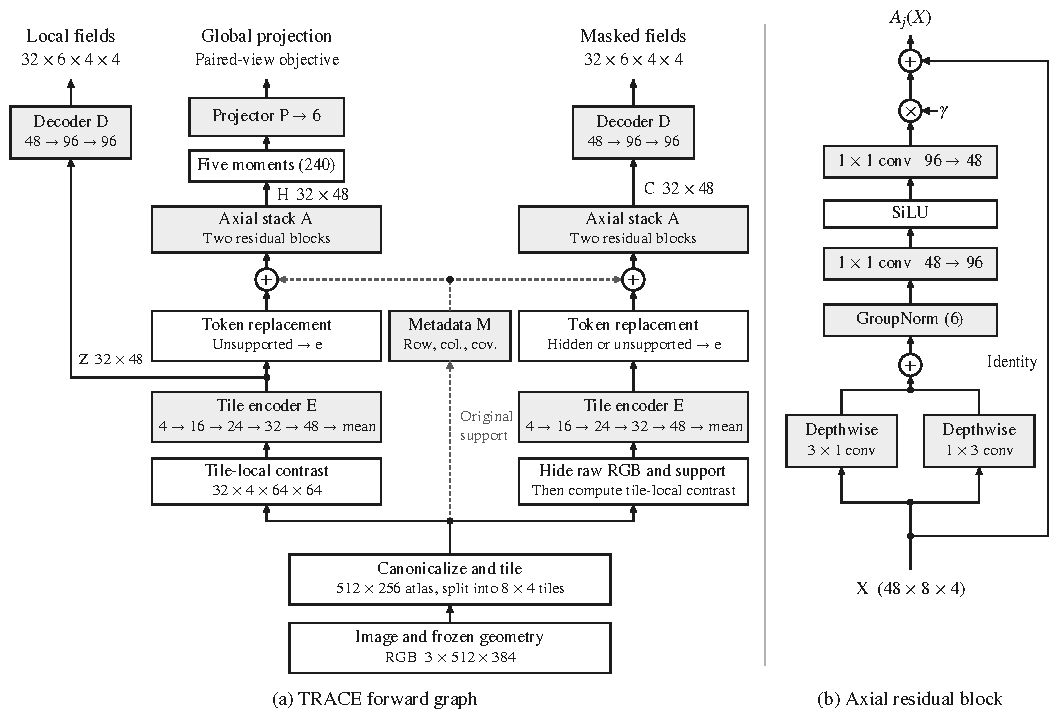
\includegraphics[width=\textwidth]{architecture.pdf}
\caption{TRACE architecture, read from bottom to top. Shading marks parameterized modules. (a) Repeated $E$, $A$, and $D$ symbols denote shared modules. Dashed arrows carry original support and its metadata. The learned mask token is $e$. The five moments use coverage-derived mass. (b) One axial block with per-channel scale $\gamma$ and an identity skip. The two blocks have distinct weights. Batch dimensions are omitted.}\label{fig:architecture}
\end{figure*}

\begin{table*}[!t]
\caption{Exact trainable TRACE layers verified against the executed model source. Tensor sizes omit the batch axis. Encoder shapes are per tile. All convolutions and linear layers include bias. Convolutions use zero padding, GroupNorm uses affine parameters with $\epsilon=10^{-5}$, and both heads use SiLU only after their first linear layer.}\label{tab:architecture}
\centering\small
\begin{tabularx}{\textwidth}{l l L r}\toprule
Layer & Input $\rightarrow$ output & Operation & Parameters\\\midrule
Encoder 1 & $4\times64\times64\rightarrow16\times32\times32$ & $3\times3$ conv., stride 2, pad 1, GroupNorm(4), SiLU & 624\\
Encoder 2 & $16\times32\times32\rightarrow24\times16\times16$ & Same kernel, stride, padding, normalization and activation & 3,528\\
Encoder 3 & $24\times16\times16\rightarrow32\times8\times8$ & Same kernel, stride, padding, normalization and activation & 7,008\\
Encoder 4 & $32\times8\times8\rightarrow48\times4\times4$ & Same blocks, followed by spatial mean to 48 channels & 13,968\\
Metadata & $32\times3\rightarrow32\times48$ & Shared linear projection of row, column, and coverage & 192\\
Mask token & $48$ & One learned vector, zero initialized & 48\\
Axial blocks 1 and 2 & $48\times8\times4\rightarrow48\times8\times4$ & Per block: sum $3\times1$ and $1\times3$ depthwise convs. (48 groups, stride 1, pad $(1,0)$ and $(0,1)$), GroupNorm(6), $1\times1$ conv. $48\rightarrow96$, SiLU, $1\times1$ conv. $96\rightarrow48$, learned scale and skip & $2\times9,888$\\
Tile decoder & $48\rightarrow96\rightarrow96$ & Shared two-layer MLP, reshape output per tile to $6\times4\times4$ & 14,016\\
Global projector & $240\rightarrow48\rightarrow6$ & Two-layer MLP on weighted full-context moments & 11,862\\\midrule
\multicolumn{3}{l}{Total trainable texture parameters} & 71,022\\\bottomrule
\end{tabularx}
\end{table*}

Table~\ref{tab:architecture} specifies the trainable layers. Each context path replaces tiles below 0.25 predicted coverage with the learned mask token. The masked path also replaces intentionally hidden tiles. Both paths add the same projected row, column, and coverage metadata and reuse the axial stack. Its two residual blocks operate on $48\times8\times4$ grids and initialize each learned residual scale to 0.1.

Coverage is normalized within each supported band and then equally across supported bands to yield nonnegative masses $m_t$ with $\sum_t m_t=1$. The recorded local mean is $\sum_t m_t Z_t$, and the full-context mean is $\sum_t m_t H_t$.

The actual global descriptor contains five moments of $H$. Coordinates $y$ and $x$ are the fixed linearly spaced values from $-1$ to $1$ on the eight rows and four columns. With
\begin{equation}
 b_t=[1,y_t,x_t,y_tx_t,y_t^2-1/3],
\end{equation}
the descriptor concatenates $\sum_t m_t b_{tk}H_t$ for $k=1,\ldots,5$, yielding 240 dimensions. The constant $1/3$ is source-defined; the discrete basis is not assumed orthogonal under each image's masses. A $240\rightarrow48\rightarrow6$ projector supplies the paired-view diversity objective. It does not feed the local decoder.

\subsection{Masking, Objective, and Original Selection}\label{sec:training}
Two deterministic image/view-addressed photometric views vary brightness, contrast, and gamma in $[0.9,1.1]$, while targets remain those of the clean atlas. A separate plan hides one supported tile in a band when at least two exist, for at most eight hidden tiles. Hidden raw RGB and observation support are removed \emph{before} preprocessing and encoding. A learned mask token and the permitted position/coverage metadata then enter the context blocks, producing $C$. The masked prediction $D(C)$ is scored on hidden supported cells. Clean targets, annotation ignore masks, and full-path encodings are not context inputs. However, the fixed predicted geometry was computed from the full image; the masking boundary is conditional on that geometry and is not a claim of image-level causal occlusion.

The loss is
\begin{equation}\label{eq:loss}
\begin{split}
\mathcal{L}={}&\mathcal{L}_{\mathrm{local}}+\mathcal{L}_{\mathrm{mask}}
 +0.1\mathcal{L}_{\mathrm{pair}}\\
 &+0.1\mathcal{L}_{\mathrm{var}}+0.01\mathcal{L}_{\mathrm{cov}}.
\end{split}
\end{equation}
Reconstruction uses Smooth L1 with transition $\beta=0.1$ on standardized fields. Valid-pixel counts weight cells, channels are averaged within images, and available images are averaged equally. The two views' terms are averaged. The pair term is mean squared error between six-dimensional projected vectors. With unbiased sample covariance $\Sigma$ ($n-1$ denominator), the variance term averages $\max(0,0.1-\sqrt{\Sigma_{j,j}+10^{-4}})$ over channels. The covariance term is $\sum_{j\ne k}\Sigma_{j,k}^2/(6\cdot5)$. The VICReg-inspired diversity losses require at least seven eligible rows for six-dimensional centered variation.

TRACE uses AdamW with learning rate 0.001, weight decay 0.0001, gradient clipping at one, FP32 arithmetic, and no scheduler or gradient scaler. One seed is run for 60 epochs and 49 updates per epoch. Each epoch has 386 primary image draws and six deterministic padding draws, yielding 23,520 draws in total. Kaggle provides two T4 graphics processing units (GPUs): geometry-cache construction uses the second device and texture optimization the first. This is not distributed data-parallel training.

Three controls predict hidden descriptors: the training channel mean, the training position mean, and the mean of visible descriptors in the same band. All are scored on the same intersection of supported hidden cells and control availability. The original validation contract requires at least 90\% primary exposure and 95\% common control coverage; at least 5\% masked improvement over \emph{each} control; at least 10\% local improvement over the position control; projector rank at least four and median standard deviation at least 0.05; local-mean and spatial-summary ranks at least four; and within-component local/spatial ranks at least two. Finite-state and frozen-geometry provenance checks also apply. Eligible checkpoints minimize masked loss divided by the strongest control loss, plus 0.1 times paired cosine distance, retaining the earliest tie. No epoch is eligible, so the selected endpoint remains unavailable. The final epoch is studied as a fixed diagnostic endpoint.

\section{Saved-Feature Aggregation Study}\label{sec:aggregation}
\subsection{Endpoint, Inputs, and Replay Boundary}
We analyze the fixed final TRACE endpoint at epoch 60, update 2,940. The retained evidence contains $Z$, $H$, and $C$ for 570 images and two recorded views, each of shape $32\times48$, together with masses, mask plans, fixed targets, target weights, and frozen decoder/projector parameters. No new photo, photometric view, geometry forward pass, image-encoder forward pass, or optimizer update is introduced. The primary intervention sweep performs 656,640 frozen decoder-token readouts. Bridge verification adds 72,960 decoder-token and 1,140 projector-vector readouts. Calling it saved-feature analysis therefore does not mean zero computation.

View 0 is the primary clean observation. View 1 is a retained sensitivity view; its appearance factors and mask plan both differ, so a change between views cannot be attributed to appearance alone. Training-only templates and scales use view 0. The validation and historical-test roles contain all 32 supported tiles per image. Two training images have missing tiles, with at least 28 supported. Fixed-grid training spectra can consequently include placeholder effects; our principal covariance interpretation uses the complete-support held-out roles.

\subsection{Nine Fixed Interventions}
For one image/view and one token layer, let $X\in\mathbb{R}^{32\times48}$, $M=\operatorname{diag}(m)$, and $B\in\mathbb{R}^{32\times k}$ be a prescribed spatial basis. The mass-weighted projection is
\begin{equation}\label{eq:projection}
 \mathcal{P}_B(X)=B(B^{\mathsf T}MB)^+B^{\mathsf T}MX,
\end{equation}
where the Moore--Penrose pseudoinverse uses relative cutoff $10^{-10}$. This reconstructs a token at every original position from the permitted spatial modes. It changes neither feature channels nor decoder parameters.

The nine interventions are: (1) original tokens; (2) one constant mode, equivalent to a global mass-weighted mean; (3) eight row-band indicators; (4) four column indicators; (5) the five source-defined spatial moments; (6) a constant plus four fixed random zero-sum orthogonal modes; (7) a train-position feature template; (8) that template plus a constant-mode residual; and (9) that template plus five residual moments. Random modes are generated once with seed 462225 using Gaussian draws, mean removal, and QR factorization. They are a dimension-matched spatial control, not an optimized random search.

Let $T$ be the unweighted per-position feature mean over supported training images, fitted separately for each layer. The final two variants are
\begin{equation}
 \widehat X=T+\mathcal{P}_B(X-T).
\end{equation}
The template is a feature statistic, not a target-fitted neural model. All held-out fitting is excluded. Bands, columns, moments, and random modes have different dimensions or structure; the analysis asks what each prescribed compression retains, not whether one has superior capacity after matched retraining.

The unchanged decoder $D$ reads each transformed $Z$ for local reconstruction and each transformed $C$ for masked reconstruction. The same supported cells, hidden cells, and train-position-control availability are used for every variant. Full-context $H$ participates in representation diagnostics and in verification of the actual global branch; it is not substituted into the local reconstruction headline.

\subsection{Loss and Retained Advantage}\label{sec:utility}
For predictions $p_{icuv}$ and standardized targets $t_{icuv}$, define Smooth L1
\begin{equation}
 h_\beta(a)=\begin{cases}a^2/(2\beta),&|a|<\beta,\\ |a|-\beta/2,&\text{otherwise},\end{cases}
\end{equation}
with $\beta=0.1$. Cell weights are valid-pixel counts on the common support. The image loss averages channels after weighted cell reduction; role-level loss averages available images equally. Thus a large tyre region does not automatically dominate a small one.

Let $L_0$ be the loss of original tokens, $L_v$ the loss under intervention $v$, and $L_{\mathrm{pos}}$ the fixed train-position target control on the same support. We report
\begin{equation}\label{eq:retention}
 R_v=\frac{L_{\mathrm{pos}}-L_v}{L_{\mathrm{pos}}-L_0}.
\end{equation}
For a positive original advantage, $R_v=1$ retains that advantage, $R_v=0$ matches the position control, and a negative value is worse than that control. It is not a classification accuracy, a proportion of physically meaningful information, or a universal information measure. Small original margins can make channel-specific $R_v$ unstable; we therefore show absolute channel losses as well.

The 21.63\% original masked-improvement headline uses the \emph{strongest declared control}, the visible-band mean, whereas~\eqref{eq:retention} consistently uses the train-position control. These denominators answer different questions and are not interchanged. The transformed tokens may also lie outside the decoder's training distribution. Their loss measures compatibility and recoverable evidence under the \emph{fixed} readout, not all information that a newly trained decoder could exploit.

\subsection{Spectral and Component Diagnostics}\label{sec:spectra}
For a role-centered image-feature matrix with covariance eigenvalues $\lambda_j\geq0$, define
\begin{equation}\label{eq:rank}
 p_j=\frac{\lambda_j}{\sum_\ell\lambda_\ell},\qquad
 \rankE=\exp\!\left(-\sum_jp_j\log p_j\right).
\end{equation}
For the saved-feature diagnostics, numerical eigenvalues below $10^{-14}$ of total energy are excluded. Original selection retains its native positive-eigenvalue treatment; no gate is recomputed with a changed rule. This is covariance-energy entropy rank. Since $\lambda_j$ is proportional to squared singular value, it differs from singular-value-weighted effective rank. Leading-energy fraction, coordinate standard deviations, and dimensions accompany it. Concatenated 1,536-dimensional tokens and pooled 48-dimensional means have different rank ceilings; their comparison is a mechanism diagnostic, not matched model performance.

We also center each conservative component separately. The between-component fraction is $1-V_{\mathrm{within}}/V_{\mathrm{total}}$, using the same covariance trace convention. This identifies where variance lies, without making component identity a permissible deployment input. In these data, class and component are confounded, so removing identity indiscriminately could also remove category-associated variation.

For a spatial decomposition, fix a single mass vector $r$ to the mean recorded training mass, normalized to sum to one. Using the same role and centering policy, let
\begin{equation}
 K_{t,u}=\frac{1}{N-1}\sum_{i=1}^{N}
 \big\langle \widetilde X_{i,t},\,\widetilde X_{i,u}\big\rangle.
\end{equation}
Then the weighted tile variance, constant-mode variance, and spatial residual obey
\begin{equation}
\begin{aligned}
 V_{\mathrm{tile}}&=\sum_{t=1}^{32} r_t\,K_{t,t},\\
 V_{\mathrm{mean}}&=r^{\mathsf T}Kr.
\end{aligned}
\end{equation}
\begin{align}
 V_{\mathrm{res}}&=\frac{1}{N-1}\sum_{i,t}r_t\left\|\widetilde X_{it}-\sum_u r_u\widetilde X_{iu}\right\|^2,\\[-3pt]
 V_{\mathrm{tile}}&=V_{\mathrm{mean}}+V_{\mathrm{res}}.\label{eq:partition}
\end{align}
Using fixed $r$ makes this identity interpretable. It differs deliberately from the per-image masses used for actual network pooling and reconstruction interventions. Diagonal and cross-position covariance contributions are retained separately.

Finally, we standardize each global feature coordinate using only training-view-0 mean and standard deviation, with floor $10^{-3}$. The inverse transformation is checked. A rank change under this invertible rescaling demonstrates sensitivity to coordinates; it cannot add information to the vector.

\subsection{Exploratory Mask-Layout Association}
After observing high rank in masked tokens, we added a separate diagnostic comparing recorded 32-position hidden indicators with full-context $H$, masked-context $C$, their difference $C-H$, and the actual projector output. For centered Gram matrices $A$ and $B$, linear CKA is
\begin{equation}
 \operatorname{CKA}(A,B)=\frac{\langle A,B\rangle_F}{\|A\|_F\|B\|_F}.
\end{equation}
Component-centered versions remove component means before constructing the Grams. This is an association with a deterministic image-addressed plan, not a randomized masking experiment. CKA is not an explained-variance percentage. The actual projector reads full-context $H$, so a strong association in $C-H$ cannot by itself explain the projector's failed diversity gate.

\section{Decoder-Aware Spatial Budget Audit}\label{sec:budget}
The nine interventions establish that spatial layout matters. Their numbers of modes differ, and the original comparison has one random basis. We therefore ask whether a spatial basis that accounts for the frozen decoder retains more task utility at the same number of image-dependent coefficients. We also measure how much loss changes solely when the order of projection and decoding is reversed.

\subsection{A Common Affine Spatial Codec}
Let $X_i\in\mathbb{R}^{32\times48}$ be one token grid, $T$ a shared train-position template, and $S=\operatorname{diag}(\sqrt{r})$ for the normalized mean training mass $r$. The fixed-mass protocol uses one $S$ across images and methods. It complements the per-image weighted projections in Section~\ref{sec:aggregation}. Every basis has an orthonormal prefix $Q_k$ with the mandatory first column $u=S\mathbf{1}$. The other columns lie in $u^\perp$. Define
\begin{align}
 P_k &= S^{-1}Q_kQ_k^\mathsf{T}S,\\
 \widehat X_i &= T+P_k(X_i-T).
\end{align}
The image-dependent code is $Q_k^\mathsf{T}S(X_i-T)$, with $48k$ real scalars. The template, basis, and weights are shared. We compare coefficient counts without assuming quantization, entropy coding, or a speed gain. Full support holds for every held-out image. Two incomplete-support train images contribute to the supported-position template but are excluded from the spatial eigensystem.

\subsection{Optimal Subspace for Each Training Surrogate}
Let $A_i=X_i-T$ and let $E$ be any orthonormal basis for $u^\perp$. For training snapshot residuals $F_i\in\mathbb{R}^{32\times d}$, form the $31\times31$ matrix
\begin{equation}
 C_F=\sum_{i\in\mathcal T} a_i
 (E^\mathsf{T}SF_i)(E^\mathsf{T}SF_i)^\mathsf{T},
\end{equation}
where $a_i$ is the nonnegative normalized weight of a full-support training image. If $U$ contains $k-1$ orthonormal columns in the 31-dimensional coordinate space, then $Q_k=[u,EU]$. The squared residual cost in snapshot space is
\begin{equation}
 \sum_i a_i\|S(I-P_k)F_i\|_F^2
 =\operatorname{tr}(C_F)-\operatorname{tr}(U^\mathsf{T}C_F U).
 \label{eq:spatial-optimum}
\end{equation}
The equality follows by orthogonality of $u$ and $E$ and idempotence of $UU^\mathsf{T}$. The Rayleigh--Ritz principle gives a minimum by taking the leading $k-1$ eigenvectors of $C_F$. The optimum residual equals the sum of the omitted eigenvalues. This is an exact statement about each declared squared surrogate under the fixed spatial mass and mandatory mean. It makes no optimality claim for held-out Smooth L1 loss.

We fit three bases under this common rule. \emph{Token PCA} uses $F_i=A_i$ and minimizes token error. \emph{Jacobian PCA} uses $F_i=A_i J^\mathsf{T}$, where $J$ is the analytic Jacobian of the frozen decoder at the shared anchor $r^\mathsf{T}T$. For an affine decoder, this is the exact output-space squared residual objective. For the nonlinear decoder it is a shared linear approximation. \emph{Decoded PCA} uses $F_i=D(X_i)-D(T)$ and minimizes the squared residual of projecting these frozen output snapshots. At evaluation, all three fitted bases project the same input tokens before decoding. Decoded PCA therefore uses the same $48k$ image-dependent scalars as token PCA. Both decoder-aware fits use decoder weights and saved train tokens as their sole data sources.

We compare the fits with separable discrete cosine transform (DCT) modes, the original five spatial moments at $k=5$, and 16 seeded random orthonormal bases in $u^\perp$. DCT frequencies are ordered by squared normalized spatial frequency with lexicographic ties, then orthogonalized in the fixed mass metric. We report $k\in\{1,2,4,5,8,16,32\}$ including the constant. At $k=1$ and $32$, all complete basis families are equivalent. The main fit weights 384 full-support training images equally, using the original supported-position template from 386 train images. The sensitivity audit fits both the template and eigensystem under equal component weight and after separately removing each of the six training components. The mass remains fixed. These are perturbations of basis construction, not new independent cohorts.

\subsection{Exact Loss Accounting Across the Decoder}
To separate what is lost in the chosen spatial subspace from what changes because the decoder is nonlinear, define
\begin{align}
 \widehat Y_{\mathrm{pre}} &= D\big(T+P_k(X-T)\big),\\
 \widehat Y_{\mathrm{post}} &= D(T)+P_k\big(D(X)-D(T)\big).
\end{align}
For an affine pointwise decoder these are identical, because spatial projection acts on rows and the linear decoder on feature channels. They can differ for the measured SiLU decoder. Holding the scoring support and target fixed, the signed task-loss change is exactly
\begin{equation}
\begin{split}
 L(\widehat Y_{\mathrm{pre}})-L(D(X))
  ={}& L(\widehat Y_{\mathrm{post}})-L(D(X))\\
     &+L(\widehat Y_{\mathrm{pre}})-L(\widehat Y_{\mathrm{post}}).
\end{split}\label{eq:order}
\end{equation}
The first term measures output-space compression under the same spatial basis. The second measures the effect of changing the order. Both can have either sign. Output-first requires $96k$ coefficients and serves as a diagnostic with a different scalar budget.

Each scalar Smooth L1 derivative has magnitude at most one. For normalized pixel weights $w_j$ and predictions $Y,Y'$ on the same support, the mean value theorem gives
\begin{equation}
 \left|L(Y)-L(Y')\right|\leq\sum_j w_j|Y_j-Y'_j|.
\end{equation}
This applies both to the total task-loss change and to the order term. We check both bounds on every scored image and report signed change alongside output drift. The protocol fixes the primary comparison at five modes, the local branch and clean view~0, with validation and historical test kept separate. The masked branch and the second recorded view probe the scope of the result. All checks are paired by image. Each held-out role has only two components for cross-tyre inference.

\subsection{Subspace and Readout Sensitivity}\label{sec:readout-method}
Let $B_i=E^\mathsf{T}S(X_i-T)$. The token and Jacobian covariances share the form $\sum_i a_i B_i W B_i^\mathsf{T}$ with channel metric $W=I$ and $W=J^\mathsf{T}J$, respectively. If the cross-position second moments factor into a spatial coefficient and a common channel matrix, then changing $W$ scales the spatial covariance by a common factor. For a positive factor, the leading spatial eigenspace is unchanged. This is a sufficient condition for identical subspaces. We measure the actual overlap without assuming separability. For two four-column orthonormal residual bases $U_1,U_2$, the singular values of $U_1^\mathsf{T}U_2$ give the cosines of the principal angles. The mean of their squared cosines excludes the constant mode shared by all methods.

We test the near-affine explanation separately. At all 32 template positions and all 12,288 full-support training tokens per branch, we measure the relative Frobenius difference between the analytic Jacobian and the one at the shared anchor. We also compare exact decoder residuals $D(X_{i,t})-D(T_t)$ with $(X_{i,t}-T_t)J^\mathsf{T}$ and with a position-specific linearization about $T_t$. The relative error is the fixed-mass weighted residual norm divided by the exact decoder-residual norm.

As a readout sensitivity control, we fit one shared affine decoder per branch to uncompressed view-0 training tokens. For each of the 16 cell locations within a tile, weighted ridge least squares maps 48 channels to six standardized descriptors. The weights are the valid-pixel counts on the common scoring support, normalized to sum to one within the fit for that cell. The ridge coefficient is $10^{-3}$, and the intercept is unpenalized. We freeze each fitted readout and apply it to the original tokens and all five-mode variants. Retention is relative to that readout's own uncompressed loss and the same position control. This changes the downstream readout at epoch 60 and leaves the representation and spatial bases fixed.

\section{Results}\label{sec:results}
\subsection{Dense Agreement Does Not Resolve Proxy Transfer}
Table~\ref{tab:trajectory} and Fig.~\ref{fig:classification} summarize the development context. Across the three validation-selected TREAD-ONE seeds, historical-test mean Dice averages 97.978\% and human point MAE 1.189\% of image width. Observed-class BA averages only 34.146\%; the selected seed values are 50.000\%, 2.439\%, and 50.000\%. All three miss every low-category image (0/62). The exported TREAD-ONE checkpoint remains seed 3, epoch 20, chosen by the recorded validation rule. Its availability as an application component is not evidence that its proxy predictions generalize.

\begin{table*}[t]
\caption{Development context on fixed allocations. Selected endpoints follow each original validation rule; final means epoch 60. BA is observed-class balanced accuracy on the 103-image historical test. These serial experiments are not a factorial ablation.}\label{tab:trajectory}
\centering\small
\begin{tabularx}{\textwidth}{LllrrL}\toprule
Experiment & Fits & Endpoint & Val. BA (\%) & Hist. BA (\%) & Main observation\\\midrule
TREAD-ONE r1 & 3 & Selected, seeds 1/2/3 & 55 / 82.5 / 100 & 50 / 2.439 / 50 & Dense agreement does not imply proxy transfer.\\
Paired baseline & 1 & Selected, epoch 23 & 55.00 & 50.000 & Matched seed-1 reference.\\
Shared projection & 1 & Selected, epoch 17 & 83.75 & 17.073 & Dense point error also worsens.\\
ATLAS v1 & 1 & Selected, epoch 18 & 50.00 & 50.000 & Low $\rightarrow$ mid; grayscale/dimming sensitivity.\\
ATLAS-LC & 1 & Selected, epoch 7 & 56.25 & 50.000 & Selected NLL improves; low recall remains zero.\\
ATLAS-CONTEXT & 1 & Selected, epoch 7 & 50.00 & 50.000 & Position sensitivity without better transfer.\\
GEO & 1 & Final; selected unavailable & --- & --- & Geometry floor 60/60; representation eligibility 0/60.\\
TRACE & 1 & Final; selected unavailable & --- & --- & Local/masked utility 60/60; global diversity 0/60.\\\bottomrule
\end{tabularx}
\end{table*}

\begin{figure*}[t]
\centering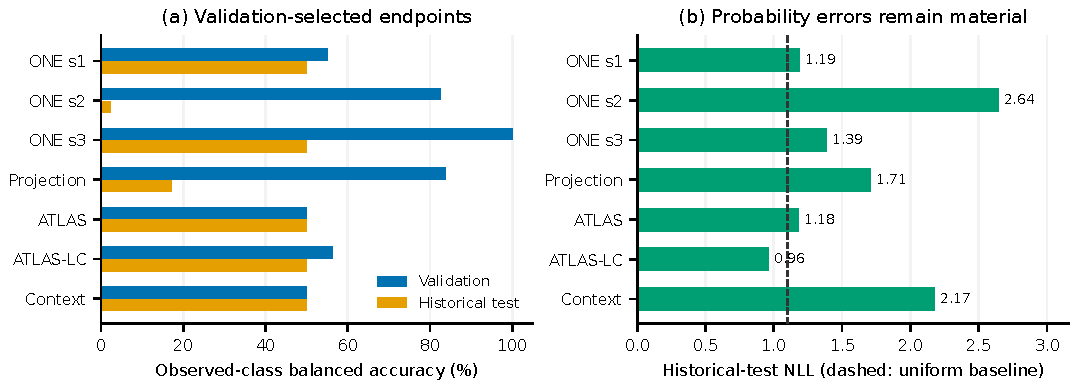
\includegraphics[width=\textwidth]{classification.pdf}
\caption{Validation-selected classifier endpoints on the same historical allocations. ONE s1--s3 are the three TREAD-ONE seeds; Projection is the paired shared-gradient candidate. Later candidates have one seed. NLL is the three-output negative log likelihood on the historical test. The dashed NLL line is the uniform three-output reference ($\ln 3$). The historical split was reused during development.}\label{fig:classification}
\end{figure*}

The shared-gradient candidate intervenes on 91.84\% of its updates but reduces selected BA from 50.000\% to 17.073\%, while human point MAE rises from 1.067\% to 1.885\% of width. This matched result does not support the intervention for this run. It also does not establish that all gradient-conflict methods fail in tyre inspection.

ATLAS, LC, and CONTEXT each retain 50\% historical BA: low recall is 0/62 and high recall 41/41. ATLAS predicts the low group as mid. LC's selected negative log likelihood (NLL) improves from 1.1783 to 0.9613, whereas CONTEXT reaches 2.1748. Probability errors therefore change despite identical endpoint BA, consistent with the need to examine more than hard decisions \cite{calibration}. LC's grayscale stability is partly by construction. CONTEXT responds to layout changes, but that response is not evidence of useful classification. These observations justify the narrower texture investigation without proving a single cause of the proxy failures.

GEO's validation geometry moves from Dice 0.9898659 and point MAE 0.0080854 of width to 0.9898623 and 0.0076622. The 5.23\% relative point reduction is about 0.163 pixels at width 384 and should not be inflated into a physical-accuracy claim. Its final masked reconstruction improves only 4.03\% over the stated mean control, below its 5\% threshold, and its projector rank is 1.0387. No GEO epoch satisfies the joint selection contract.

\subsection{TRACE Learns Local Fields but Remains Unselected}
Table~\ref{tab:trace} gives final TRACE values. Local validation loss is 0.421632 against a train-position loss of 0.663375, a 36.44\% reduction. Masked validation loss is 0.467383 against 0.691031 for the channel mean, 0.662256 for the position mean, and 0.596403 for the visible-band mean. The gain against the strongest aggregate control is 21.63\%. The historical-test counterpart is 17.85\%. Each of the 81 validation images and 103 historical-test images beats all three controls for its final clean-view recorded mask plan; 81/81 and 98/103, respectively, exceed 5\% against every control. These are within-image evidence comparisons, not independent tyre-level success rates.

\begin{table*}[t]
\caption{TRACE final clean-view reconstruction and original validation gate diagnostics. Losses are equal-image standardized Smooth L1.}\label{tab:trace}
\centering\small
\begin{tabularx}{\textwidth}{LrrLrr}\toprule
Reconstruction & Validation & Hist. test & Validation diagnostic & Value & Floor\\\midrule
Local model loss & 0.421632 & 0.412205 & Projector rank & 1.0225 & $\geq4$\\
Local position control & 0.663375 & 0.662712 & Local mean rank & 1.2296 & $\geq4$\\
Local reduction (\%) & 36.44 & 37.80 & Spatial rank & 1.2489 & $\geq4$\\
Masked model loss & 0.467383 & 0.472012 & Projector std. median & 0.0961 & $\geq0.05$\\
Masked visible-band control & 0.596403 & 0.574568 & Within local rank & 9.7824 & $\geq2$\\
Masked reduction (\%) & 21.63 & 17.85 & Within spatial rank & 11.2722 & $\geq2$\\\bottomrule
\end{tabularx}
\end{table*}

Utility, exposure, coverage, finite-state, frozen-geometry, and within-component checks pass at all 60 validation epochs. The projector and encoder/global diversity checks pass at none (Fig.~\ref{fig:training}). The final six-dimensional projector has adequate median amplitude (0.0961) but rank only 1.0225. Likewise, local and spatial pooled ranks remain 1.2296 and 1.2489. Thus amplitude is not the missing property, and the original selected endpoint remains unavailable. We analyze the final state without relaxing these gates.

\begin{figure*}[t]
\centering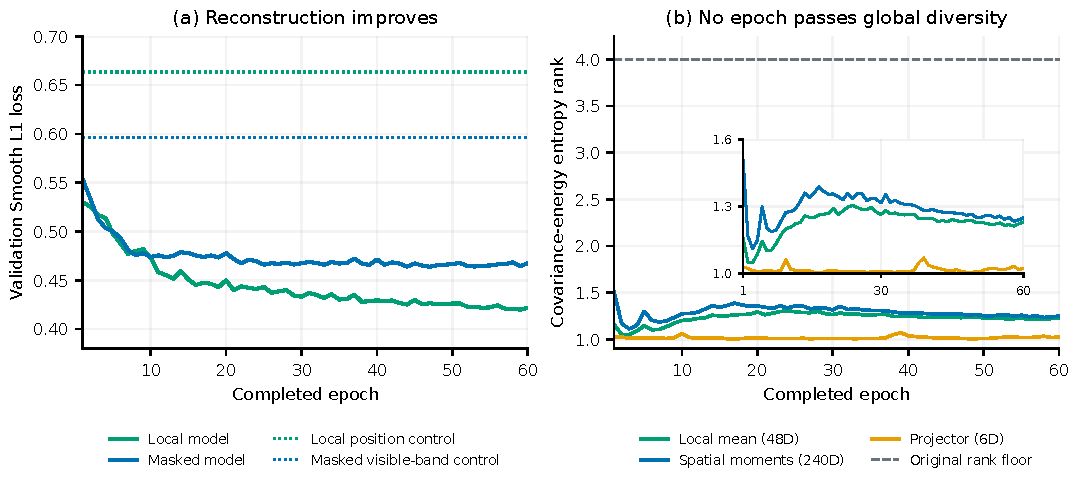
\includegraphics[width=\textwidth]{training.pdf}
\caption{All 60 recorded TRACE validation epochs. Reconstruction improves against fixed controls, while all three global rank traces remain below their original floor. The inset resolves the observed rank range. The selected endpoint is unavailable throughout; the final state is used only for the saved-feature diagnosis.}\label{fig:training}
\end{figure*}

\subsection{Equal-Budget Comparison of Spatial Bases}\label{sec:budget-results}
Table~\ref{tab:budget} reports the primary five-mode comparison, with 240 image-dependent scalars in place of 1,536 token entries. Ordinary token PCA retains 89.47\% of local validation advantage and 89.01\% on the historical test. Fixed spatial moments retain 81.71\% and 82.17\% under the same fixed mass and template. The corresponding increments are 7.76 and 6.85 percentage points, computed before rounding. Token PCA also exceeds DCT and all 16 random bases on both roles. The random ranges are 76.70--78.84\% and 76.38--79.38\%, respectively. The spatial-moments row uses a fixed training mass, while the template plus five residual moments in Table~\ref{tab:aggregation} uses image-specific coverage masses. This accounts for the small differences between the two tables.

\begin{table*}[t]
\caption{Retained position-control advantage (\%) at five modes including the constant. All methods use a shared fixed mass, position template, and 240 image-dependent input coefficients. View 0 is shown.}\label{tab:budget}
\centering\small
\begin{tabular}{lrrrr}\toprule
 & \multicolumn{2}{c}{Local} & \multicolumn{2}{c}{Masked}\\
Basis & Validation & Hist. test & Validation & Hist. test\\\midrule
\budgetrows
\bottomrule\end{tabular}
\end{table*}

\begin{figure*}[t]
\centering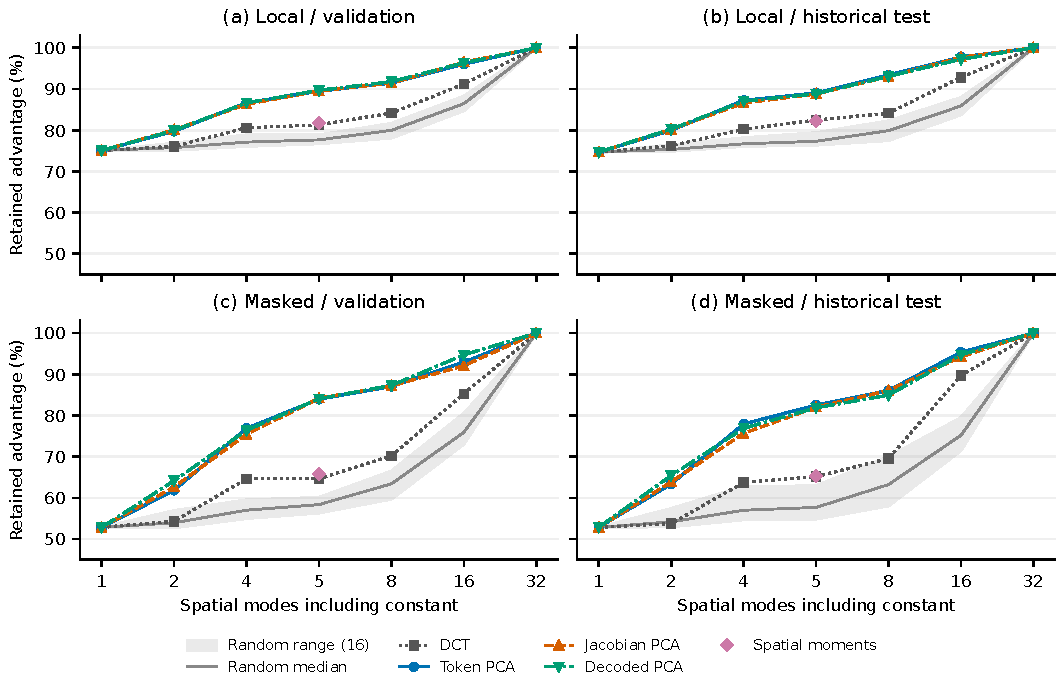
\includegraphics[width=\textwidth]{spatial_budget.pdf}
\caption{Retained advantage across the fixed spatial budget. The shaded interval is the range of 16 fixed random bases and does not represent statistical uncertainty. All methods share the one-mode and full-budget endpoints. Intermediate gaps reflect differences in the spatial basis at the same input coefficient count.}\label{fig:budget}
\end{figure*}

\begin{figure*}[t]
\centering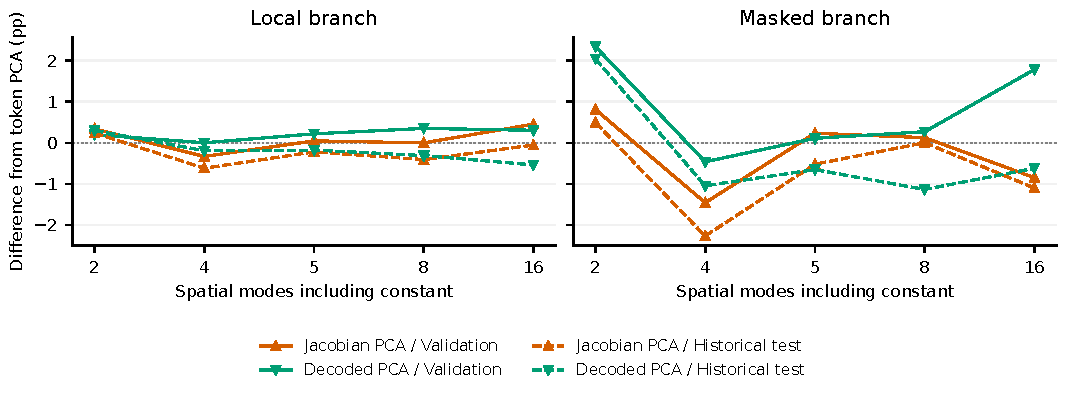
\includegraphics[width=\textwidth]{spatial_budget_differences.pdf}
\caption{Retention differences relative to token PCA at each intermediate coefficient budget. The dashed line marks equal performance. Differences are computed before rounding.}\label{fig:budget-differences}
\end{figure*}

Decoder-aware bases provide no consistent aggregate improvement over ordinary PCA. Decoded PCA improves local validation retention by 0.22 percentage points, then trails token PCA by 0.18 points on the historical test. Jacobian PCA improves masked validation by 0.23 points and trails by 0.52 points on the historical test. At five modes under view 1, the local result is nearly unchanged. Masked historical retention drops for all three fitted bases and their ordering remains token, Jacobian, then decoded PCA. The recorded views vary both appearance and mask layout. Figure~\ref{fig:budget-differences} shows the small differences concealed by the overlapping curves. At 16 modes masked validation retention is 94.72\% for decoded PCA and 92.93\% for token PCA.

The gain from fitted spatial modes also depends on the descriptor and component. At five modes token PCA reduces local validation orientation-axis loss from 0.45467 under fixed moments to 0.40166, and contrast loss from 0.62604 to 0.59896. For the historical low-proxy component it retains 80.21\% of local advantage versus 74.82\% for moments. For the historical high component the respective values are 95.42\% and 87.51\%. The remaining low/high gap shows that learned spatial modes recover some lost texture in both groups while preserving a substantial difference in retention.

\subsection{Sensitivity to Training Components and Decoder Order}
Fitting the token PCA template and basis with equal training-component weight changes five-mode local retention from 89.47\% to 89.68\% on validation and from 89.01\% to 87.92\% on the historical test. Across the six component omissions, retention spans 88.46--89.47\% and 86.45--89.01\%, respectively. All of these local values remain above the corresponding fixed-moment values. The largest historical-test reduction occurs when omitting the unresolved mid parent component, which holds the most training images. This perturbation changes both the training composition and its size, so it cannot isolate a class effect. The masked historical-test range is wider at 78.43--82.48\%. The group sensitivity is materially larger than the differences among the three five-mode PCA surrogates.

For local validation with five token PCA modes, the task-loss increase of 0.02545 separates into 0.02639 for output-space compression and $-0.00094$ for the change in order. The mean absolute difference between token-first and output-first predictions is 0.03132 on the same support. For the masked branch, this difference rises to 0.10045 while the signed order effect is $-0.00326$. Thus the nonlinear decoder changes the fields even when the signed task penalty is small. Signed loss alone would hide the extent of the prediction change. Both drift bounds hold at image level to numerical tolerance and the full-budget endpoint reproduces uncompressed predictions to within $1.5\times10^{-14}$. The independent loss reductions and source pins are described in Section~\ref{sec:repro}.

\subsection{Why the Fitted Bases Agree}\label{sec:basis-similarity}
The three fitted methods retain closely aligned spatial subspaces, consistent with their similar reconstruction results. Table~\ref{tab:angles} compares the four residual modes against token PCA. Jacobian and decoded PCA attain overlaps of 0.9773--0.9896 across branches. The same comparison for DCT and fixed moments gives overlaps of 0.4581--0.4859. Both fixed bases have at least one residual mode nearly orthogonal to the fitted subspace. The angles quantify agreement among fitted bases for this checkpoint.

\begin{table*}[t]
\caption{Subspace agreement with token PCA at five total modes. Overlap averages squared principal-angle cosines over the four residual modes, excluding the constant.}\label{tab:angles}
\centering\small
\begin{tabular}{lrrrr}\toprule
 & \multicolumn{2}{c}{Local tokens} & \multicolumn{2}{c}{Masked-context tokens}\\
Comparison basis & Overlap & Largest angle & Overlap & Largest angle\\\midrule
Jacobian PCA & 0.9896 & $7.96^\circ$ & 0.9883 & $9.02^\circ$\\
Decoded PCA & 0.9885 & $8.95^\circ$ & 0.9773 & $15.08^\circ$\\
Spatial moments & 0.4751 & $87.76^\circ$ & 0.4859 & $86.19^\circ$\\
DCT & 0.4581 & $87.21^\circ$ & 0.4712 & $86.16^\circ$\\\bottomrule
\end{tabular}
\end{table*}

The median relative Jacobian differences at the template positions are 14.57\% locally and 47.62\% for masked context. Across full-support training tokens, these increase to 31.65\% and 69.22\%. Using position-specific Jacobians lowers the relative output linearization error from 30.93\% to 25.50\% locally and from 49.93\% to 39.51\% for masked context. Thus a shared Jacobian approximates the dominant fitted spatial subspace while leaving appreciable nonlinear output residuals.

\subsection{An Affine Readout Preserves the Local Ordering}
With the train-only affine readout, five-mode token PCA retains 90.21\% and 89.91\% of its local reconstruction advantage on validation and historical test. Fixed moments retain 80.17\% and 82.07\%, while DCT retains 79.90\% and 82.42\%. All three fitted bases exceed the fixed bases and all 16 random controls in both local cohorts. Their similar retention therefore extends to this alternate decoder of the same features.

The masked branch is more decoder dependent. The uncompressed affine readout yields masked losses of 0.47434 and 0.48101, close to the original decoder's 0.46738 and 0.47201. After token PCA compression, its losses rise to 0.62830 and 0.64034. This retains 18.07\% and 10.62\% of its advantage, compared with 83.96\% and 82.51\% for the original decoder. Fixed moments and DCT fall below the position control. The fitted bases still outperform the fixed bases, but the large absolute masked retention depends on the original decoder. This comparison varies the readout at a single saved checkpoint. It provides evidence about decoder dependence and leaves checkpoint, seed, and architecture generalization open.

\subsection{Effect of the Original Aggregation Interventions}
Table~\ref{tab:aggregation} and Fig.~\ref{fig:aggregation} report all nine interventions. A global mean retains 61.14\% of the original local validation advantage and 62.12\% on the historical test. Five fixed moments retain 76.05\% and 81.89\%. A training-position template alone retains only 7.75\% and 6.31\%, whereas the template plus five residual moments retains 81.76\% and 82.17\%. Position-typical features alone therefore do not explain the original local readout's utility, but position plus image-specific residual structure preserves substantially more than a global mean.

\begin{table*}[t]
\caption{Retained advantage $100R_v$ over the train-position target control (\%). Original tokens define 100\%; negative values are worse than the control. All variants use identical target support and the unchanged decoder. These are frozen-head counterfactuals, not trained architecture comparisons.}\label{tab:aggregation}
\centering\small
\begin{tabular}{lrrrr}\toprule
 & \multicolumn{2}{c}{Local branch $Z$} & \multicolumn{2}{c}{Masked branch $C$}\\
Intervention & Validation & Hist. test & Validation & Hist. test\\\midrule
\aggregationrows
\bottomrule\end{tabular}
\end{table*}

\begin{figure*}[t]
\centering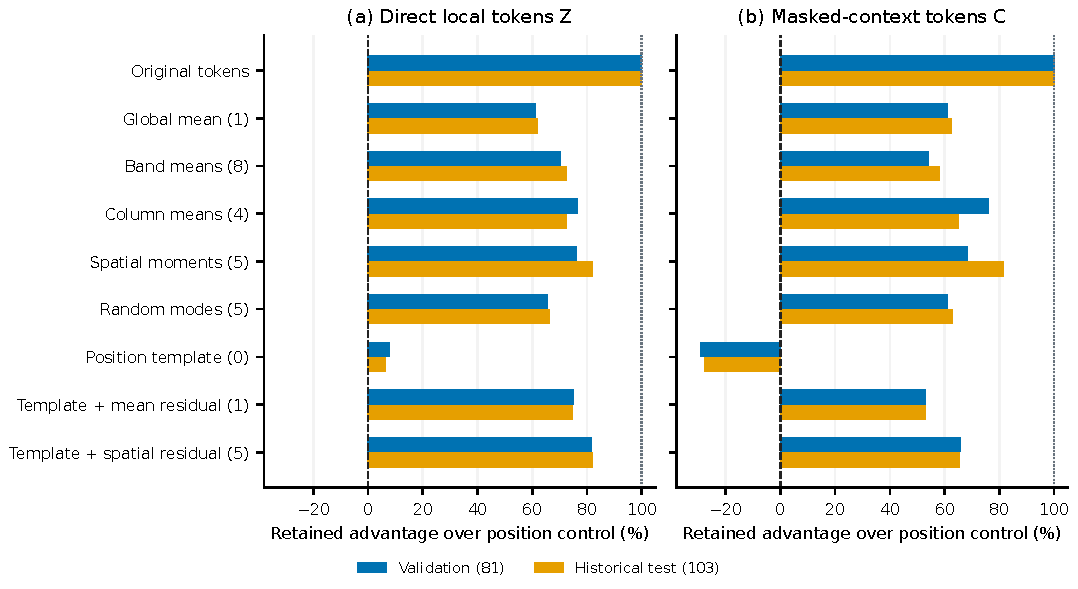
\includegraphics[width=\textwidth]{aggregation.pdf}
\caption{Retained reconstruction advantage under all nine fixed interventions. Spatial mode counts appear in parentheses. The dashed line marks zero retained advantage. A global mean loses useful local readout performance. Residual moments preserve more local utility, but they are not uniformly best for the masked task. The training-position template by itself is weak locally and worse than the position-target control on hidden cells.}\label{fig:aggregation}
\end{figure*}

Five random modes retain 65.47\% of local validation advantage, below the five prescribed spatial moments. This one fixed random basis is a control, not a distribution over random projections. Eight band means retain 70.42\%, while four column means retain 76.39\%; the number of modes alone does not order their utility.

The masked branch gives a different ordering. Four column means retain 75.90\% on validation, compared with 68.39\% for five moments, 61.23\% for a global mean, and 65.82\% for template plus residual moments. On the historical test, raw moments retain 81.55\% but the template-residual variant retains 65.29\%. The pure template is below the position-target control in both roles. No single aggregation dominates every task and component, and we do not select an architecture from the most favorable historical-test number.

\subsection{Descriptor and Component Dependence}
Figure~\ref{fig:descriptor} separates six descriptor losses from the aggregate headline. For local validation orientation-axis targets, global averaging raises loss from 0.385328 to 0.585783; residual moments recover it to 0.454548. For orientation-cross targets, the mean's loss is 0.790882, worse than the position control's 0.667389, compared with 0.616969 originally and 0.650077 for residual moments. Contrast also degrades under averaging, from 0.575280 to 0.627355, and is not substantially recovered by residual moments (0.626081). Gradient energy and occupancy are less sensitive in their absolute changes. These differences argue for descriptor-aware evidence retention rather than one global rank target. Figure~\ref{fig:qualitative} illustrates the original and compressed readouts using the lexicographically first validation image in each observed proxy class, without ranking examples by prediction quality.

\begin{figure*}[t]
\centering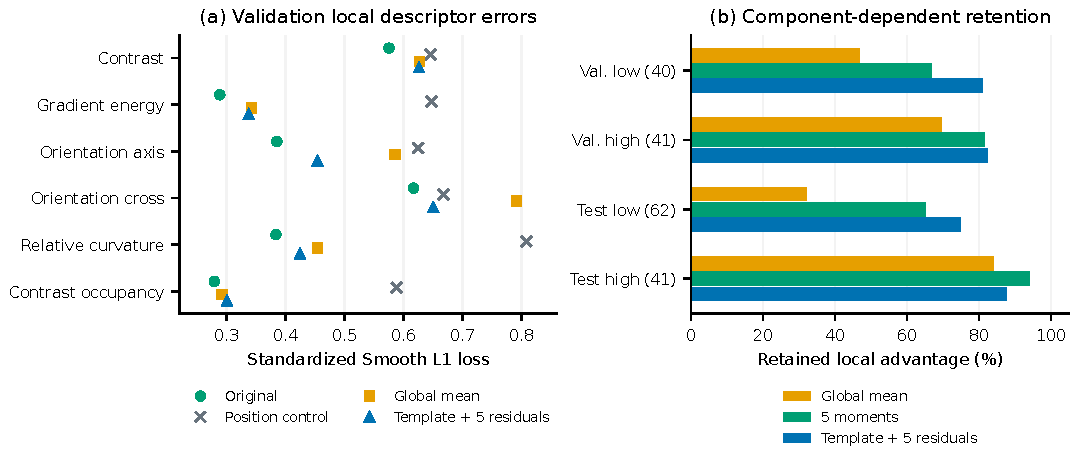
\includegraphics[width=\textwidth]{descriptor_groups.pdf}
\caption{Absolute descriptor loss and component-level local retention for clean view 0. Markers in the left panel are offset vertically within descriptor rows for legibility. Absolute losses avoid unstable percentage interpretations when the original control margin is small. The right panel shows that global averaging is more damaging for the historical low component than for the high component. Components coincide with class within each held-out role; this does not isolate a class mechanism.}\label{fig:descriptor}
\end{figure*}

\begin{figure*}[t]
\centering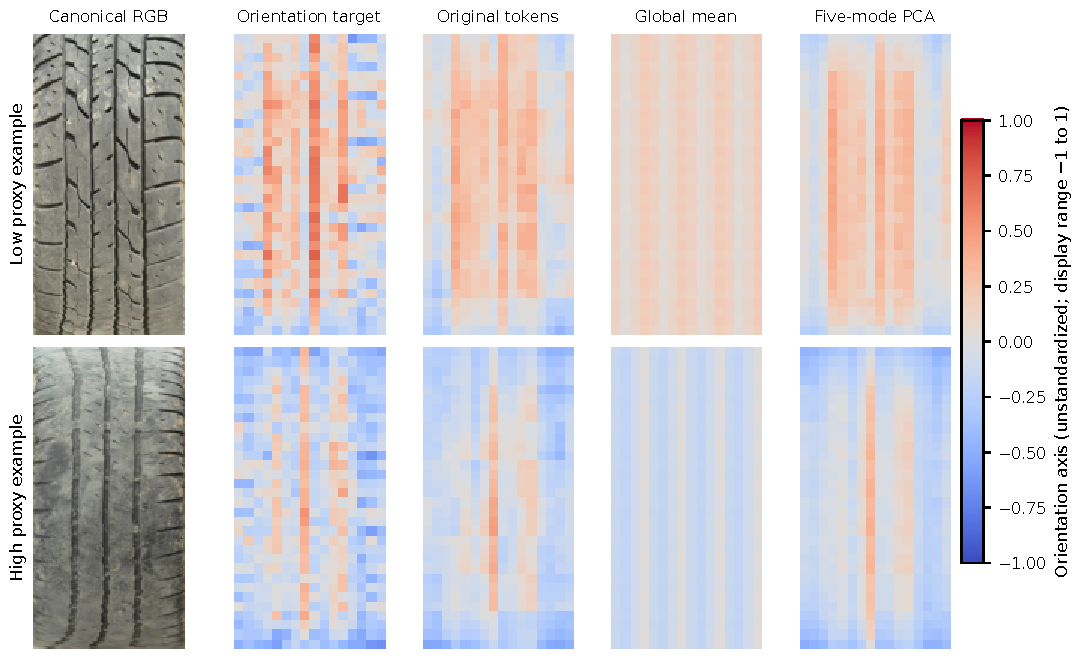
\includegraphics[width=\textwidth]{qualitative.pdf}
\caption{Two deterministic validation examples from the saved canonical atlas and orientation-axis fields. Each row uses the first image identifier in its observed proxy class, not a best/worst error selection. The target and predictions are returned to the raw descriptor scale; colors saturate outside $[-1,1]$ for display only, and unsupported cells are white. The original, global-mean and five-mode token PCA readouts use identical decoder weights. These fields describe image orientation, not groove depth or wear.}\label{fig:qualitative}
\end{figure*}

The historical-test low component retains only 32.03\% of local advantage under a mean, versus 84.02\% for high. Five raw moments retain 65.08\% and 94.13\%, while template plus residual moments retain 74.82\% and 87.52\%. For masked reconstruction the mean retains 23.16\% on low and 81.04\% on high. Such component dependence is consistent with nonuniform loss of local evidence. It does not prove that pooling caused the earlier low-class classification failures: TRACE has a different objective, the interventions are post-hoc, and identity remains confounded with class.

\subsection{Covariance Explains a Distinction, Not Semantic Quality}
Figure~\ref{fig:representation}(a) shows that concatenated local tokens have validation rank 3.4734, falling to 2.4163 after full-context mixing. The local mean has rank 1.2296, actual context moments 1.2489, and actual projector 1.0225. Hence representation concentration is already affected by context; the final averaging operation is not the only transformation implicated by these diagnostics.

After component centering, concatenated local rank is 20.090 and local-mean rank 9.782. Between-component differences account for 96.78\% of local-mean variance, 96.56\% of context-moment variance, and 99.35\% of projector variance. The few coherent component differences dominate global energy even though smaller within-component directions remain. A low total rank should therefore not be interpreted as an exactly constant vector or absence of all local structure.

The fixed training-mass partition in Fig.~\ref{fig:representation}(b) places 30.10\% of total local-token variance in the constant spatial mode, but only 4.15\% after component centering. The corresponding mean off-diagonal position correlations are 0.2731 and 0.0095. Thus most within-component token variation lies outside the constant mode and tends to cancel under averaging. The remaining 95.85\% is a variance fraction, \emph{not} a fraction of useful wear information. Reconstruction measurements, rather than this covariance identity alone, establish the narrower loss of fixed-readout utility.

\begin{figure*}[t]
\centering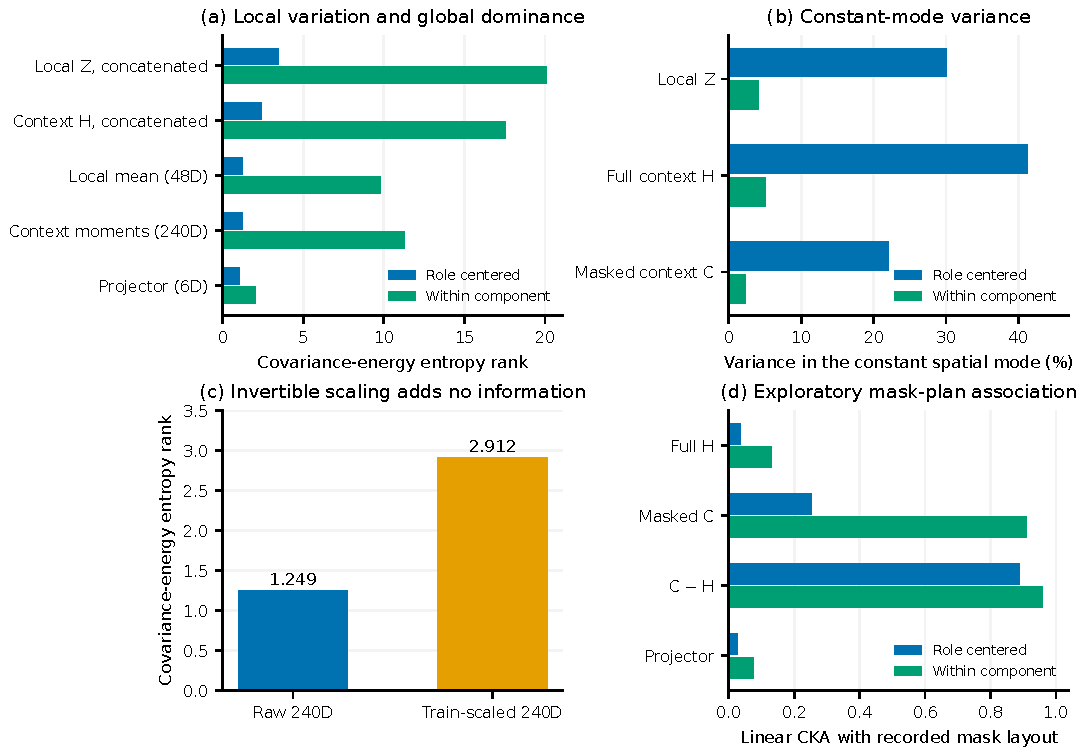
\includegraphics[width=\textwidth]{representation.pdf}
\caption{Validation representation diagnostics for clean view 0. (a) Total and within-component covariance-energy entropy ranks have different interpretations and dimensional ceilings. (b) The fixed train-mass partition isolates the constant spatial mode. (c) Invertible training-only coordinate scaling changes rank without adding information. (d) Exploratory CKA identifies strong mask-layout association in masked-context differences; it is not a proportion of explained variance.}\label{fig:representation}
\end{figure*}

Training-only coordinate scaling raises context-moment rank from 1.2489 to 2.9120 while preserving invertibility; local-moment rank rises from 1.4558 to 3.3313. These values do not replace the original ranks or selection decisions. They demonstrate why a metric improvement obtained by rescaling would not by itself show a more informative representation.

\subsection{Exploratory Mask-Layout Result}
Masked-context concatenation has validation rank 15.3126, much higher than full context. However, linear CKA between the recorded mask plan and $C-H$ is 0.8879 overall and 0.9575 after component centering. Masked context itself has within-component CKA 0.9092, compared with 0.1297 for full context. The historical-test $C-H$ values are similarly high (0.9047 overall and 0.9600 within component). These associations indicate that high masked-token diversity can strongly reflect which positions were hidden.

All validation and historical-test images hide eight tiles, so their mean hidden fraction is constant; the relevant variable is layout, not mask count. The actual projector has much lower mask association (validation CKA 0.0272 overall, 0.0760 within component) and reads full context. We therefore do not attribute its low rank to mask noise. The addendum instead shows that counting diverse masked features as semantic evidence would be premature.

\Needspace{8\baselineskip}
\section{Discussion and Limitations}\label{sec:discussion}
\subsection{Local Utility and Global Diversity Are Separate Properties}
TRACE separates useful local prediction from broad global diversity. Its local and hidden-cell heads read $Z$ and $C$ directly, bypassing the global descriptor and projector. Reconstruction success can therefore coexist with a failed global gate.

The untemplated mean preserves about three fifths of local advantage. With a shared position template, five fitted modes preserve close to nine tenths on both roles. This finding supports testing spatial summaries against an ordinary PCA baseline before adding decoder-aware complexity. In this setting, the three squared fitting objectives give very similar five-mode task retention, even though they optimize different quantities. Group perturbations are larger than the surrogate differences. A local validation lead of a fraction of a percentage point should therefore carry little weight in model selection.

Averaging favors coherent variation across positions, dominated here by component differences. Much within-component variation cancels. Intervention losses show that some discarded variation is useful to the descriptor decoder; other variation may reflect illumination, viewpoint, noise, or geometry artifacts. The data do not assign those sources a physical-wear meaning.

\subsection{What Would Justify a Future Revision?}
A compact branch can be tested against the five-mode spatial PCA baseline for incremental contrast and orientation utility. The test should preserve the visible-input masking boundary and check geometry separately. Because the current analysis projects representations of one frozen model, a trained decoder could change the ranking. The signed order term and absolute drift provide separate checks if the decoder is refitted.

This implication does not select a new objective or model. The cycle closes with its original unselected status. A future protocol must distinguish reconstruction improvement from transfer, physical measurement, and useful operator decisions.

\subsection{Limits of the Evidence}
The collection has twelve recorded tyres, six conservative training components, and two held-out components per role. The mid category contributes many training images but appears in neither held-out role. Tyre identity and mileage proxy are therefore confounded in each held-out split. Conservative merging addresses uncertainty in the provenance of related training images.

The historical test was inspected repeatedly. The nine interventions were fixed before their calculation, but the question follows observed failures. No prospective confirmation or external deployment cohort is available, and later candidates have one seed. Serial model differences therefore cannot establish seed-robust causal effects.

A fixed decoder can be sensitive to interventions outside its training distribution. Our order decomposition is an accounting identity for a specified projection and template. Its output-space reference uses twice as many scalar coefficients, and neither term measures mutual information or the best performance attainable by a refitted decoder. Concatenated and pooled spectra also differ in dimension, while component centering uses diagnostic group information unavailable to generic inference.

Canonical resampling depends on image-space geometry and heterogeneous annotations. Its atlas aligns visible structures across images. It supplies no metric scale for the height of a groove floor relative to the adjoining tread surface.

\subsection{Implications for Camera-Based Groove Depth}
The audit identifies which representations preserve visible rib and groove orientation. This is relevant to designing the front end of an optical measurement system. A single image admits ambiguity between scene scale, perspective, reflectance, and illumination \cite{eigondepth}. A metric groove-depth study would need calibrated capture, paired groove measurements in millimeters at matched positions, and evaluation on independent tyres. An optical cross-section method with scale calibration, such as TireEye \cite{tireeye}, illustrates the distinction. Depth recovery, absolute error, and calibration stability were outside the measurements reported here.

Finally, deterministic masking, an exploratory CKA addendum, and jointly changed view-1 photometry/layout limit causal attribution. Spectral concentration, mask association, and reconstruction utility require separate reporting. The evidence is application-specific, rather than a general proof about pooling or self-supervised learning.

\section{Reproducibility and Evidence Availability}\label{sec:repro}
All reductions use fixed data roles and recorded TRACE inputs. The published review reconstructs the 2,940 training objectives and 60 validation decisions. The aggregation audit uses 249 pinned native and metadata inputs, checks agreement with the original decoder, and independently reduces the derived predictions. The matched-budget audit checks full-budget reconstruction, Jacobians by finite differences, and the omitted-eigenvalue identities. The affine sensitivity analysis retains 25,080 paired per-image losses for independent reduction. These checks establish computational consistency on the saved evidence.

The public project archive contains the pinned \href{https://huggingface.co/datasets/Shanmuk4622/tyre-wear-study/tree/510cbc827337cbc963562c798811226326dc7c0c}{TRACE training record} and \href{https://huggingface.co/datasets/Shanmuk4622/tyre-wear-study/tree/7672729fdb1ccd0f55b565c1d60e8a50c6be078e}{completed review}. The companion materials include analysis scripts, compact direct CSV results, and SHA-256 receipts with exact versions. Detailed new prediction and affine derivatives are retained locally. Earlier internal work shares photographs and task components with this study.

\section{Conclusion}\label{sec:conclusion}
We introduced a matched-budget audit for the texture evidence used by a frozen decoder. A shared position template and constant mode allowed us to compare three train-fitted spatial bases against fixed and random bases. At 240 input coefficients, ordinary token PCA retained 89.47\% of local validation advantage and 89.01\% on the historical test. These values exceed the fixed-moment baselines by 7.76 and 6.85 percentage points before rounding.

The decoder-aware bases closely overlap the token PCA subspace despite substantial Jacobian variation. An affine readout preserves the advantage of fitted bases for local reconstruction, while masked retention drops sharply. Reversing the order of decoding and projection also substantially changes masked descriptor fields despite a small signed loss effect. Together these results distinguish shared spatial structure from the decoder's effect on task utility.

The results are retrospective and specific to TRACE, six image descriptors, and the available tyre components. The original selection rule still yields no eligible checkpoint. The audit provides a reproducible way to test how proposed summaries preserve local texture evidence before attributing utility to a global representation.

\FloatBarrier
\section*{Acknowledgment}
\href{https://openai.com/codex/}{OpenAI Codex} assisted in drafting and editing the abstract, Sections I--X, and figure captions. It also assisted with LaTeX and with code for the spatial-budget, reviewer, and figure analyses. The figures use recorded measurements, existing tyre photographs, and the source-defined architecture.
\bibliographystyle{IEEEtran}
\bibliography{references}
\begin{IEEEbiography}[{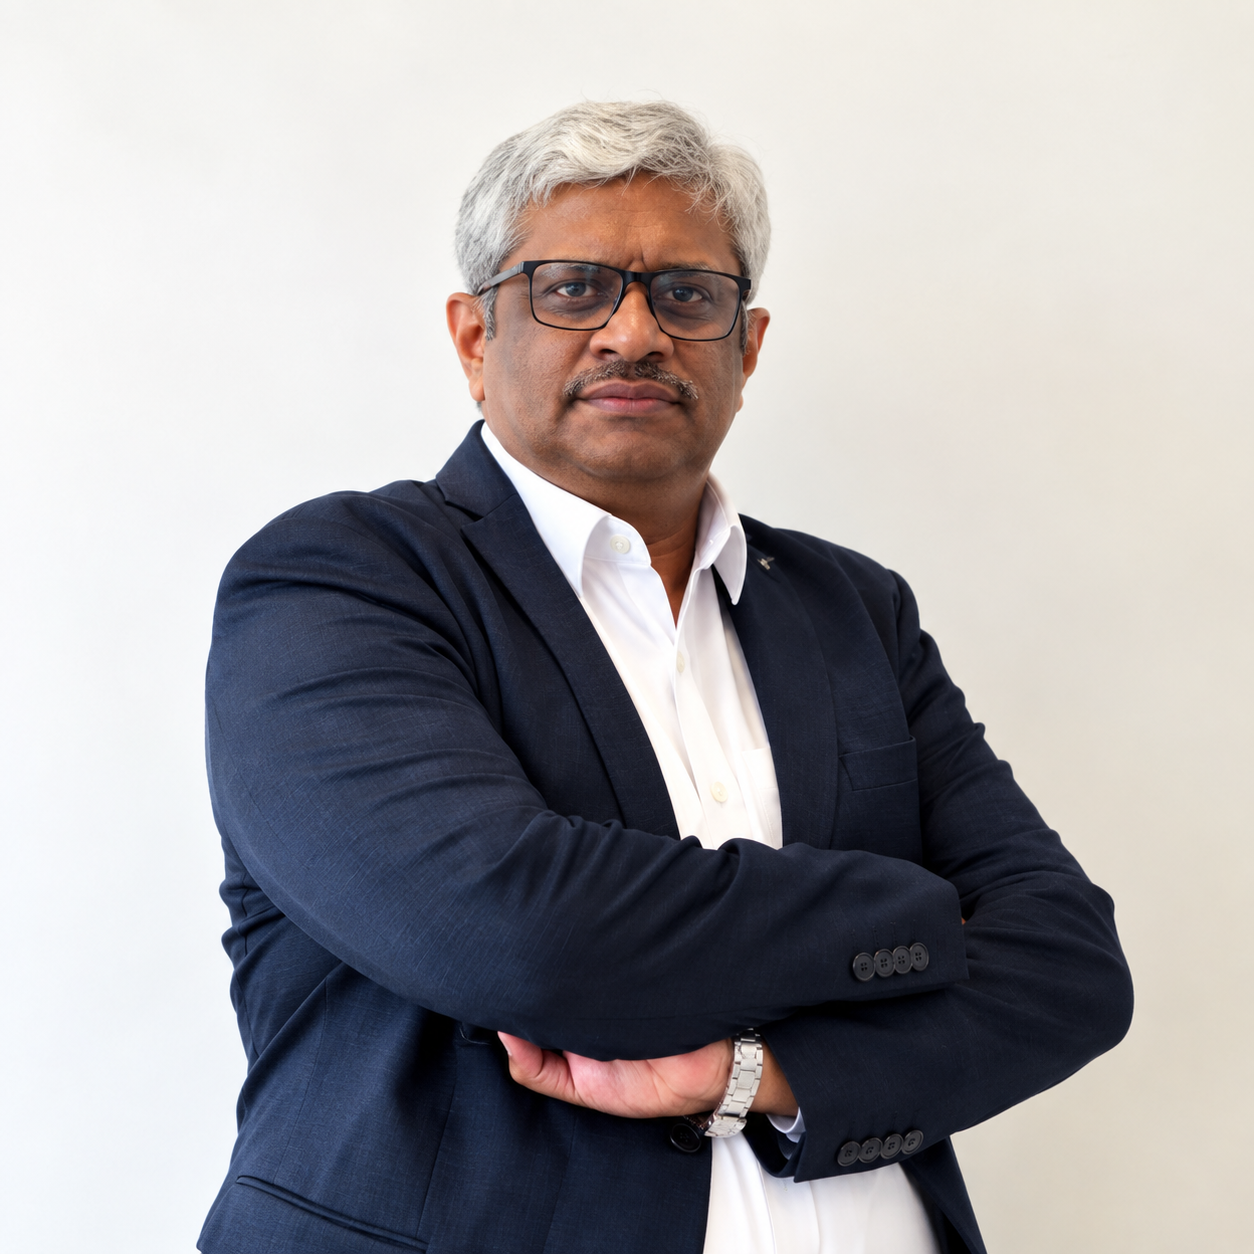
\includegraphics[width=1in,height=1.25in,clip, keepaspectratio]{a1.jpg}}]{Edara Sreenivasa Reddy} is currently a Professor (HAG) with the School of Computer Science and Engineering, VIT-AP University, Amaravati, India. He has more than 34 years of academic experience and 18 years of research experience. During his academic
career, he has served in several teaching and administrative positions, including Assistant Professor, Associate Professor, Professor, Senior Professor, Principal, Dean, and Vice-Chancellor.

He has published more than 125 Scopus-indexed journal articles, authored 12 books, contributed 12 chapters to edited research volumes, and obtained 12 patents. Under his supervision, 46 Ph.D. scholars and two M.Phil. scholars have completed their degrees. His research interests include artificial intelligence, machine learning, deep learning, generative artificial intelligence, large language models, and quantum computing.

Prof. Reddy is an NVIDIA University Ambassador for
deep learning and an NVIDIA-certified coach for generative artificial intelligence and large language models. He has also completed professional certification in quantum computing from IBM. He received the Best Computer Science Teacher Award from the Indian Society for
Technical Education. He is a Fellow of the Computer Science Research Council, USA, and an Honorary Fellow of the Academy of Science, Technology and Communications. He is a Senior Member of IEEE and a member of the Indian Society for Technical Education.

\end{IEEEbiography}

\begin{IEEEbiography}[{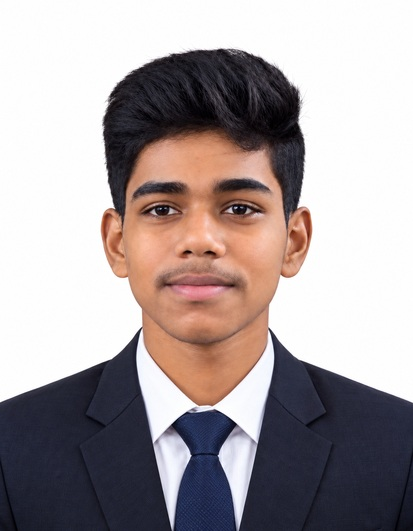
\includegraphics[width=1in,height=1.25in,clip, keepaspectratio]{a2.jpg}}]{Shanmukesh Bonala} is currently pursuing the B.Tech. degree in computer
science and engineering with VIT-AP University,
Amaravati, India. His research interests include artificial intelligence, computer vision, deep learning, model optimization, and energy-efficient artificial intelligence.

He has contributed to research and development projects in artificial intelligence and computer vision and has published research datasets through IEEE DataPort. His work focuses on the development of scalable and reproducible artificial-intelligence systems. He is an IEEE
Student Member.
\end{IEEEbiography}

\EOD
\end{document}
